\documentclass[twocolumn]{IEEEtran}
\usepackage{graphicx}
\usepackage[utf8x]{inputenc}
\usepackage{times}
\usepackage{amssymb,amsfonts}
\usepackage{pict2e}
\usepackage{float}
\usepackage[all]{xy}
\usepackage{graphics,graphicx,color,colortbl}
\usepackage{subfigure}
\usepackage{wrapfig}
\usepackage{multicol}
\usepackage{cite}
\usepackage{url}
\usepackage[tbtags]{amsmath}
\usepackage{amsmath,amssymb,amsfonts,amsbsy}
\usepackage{bm}
\usepackage{listings}
\usepackage{algorithm}
\usepackage{algorithmic}
\usepackage[centerlast, small]{caption}
\usepackage[colorlinks=true, citecolor=black, linkcolor=black, urlcolor=black, breaklinks=true]{hyperref}
\hyphenation{ele-men-tos he-rra-mi-en-ta cons-tru-yen trans-fe-ren-ci-a pro-pu-es-tas si-mu-lar di-fe-ren-cia}
\renewcommand{\refname}{Referencias}

\begin{document}
\title{Diseño e Implementación de un arreglo de antenas tipo parche con los patrones de Suma/Diferencia en la banda \textit{ISM} de $5.8\ GHz$.}
%Project 2: Design and Implementation of a Patch Array with Sum/Difference Patterns at the ISM 5.8GHZ band.
\author{David Ricardo Martínez Hernández Código: $261931$\\
	Jairo Andrés Neuta Bernal Código: $261227$\\
	Oscar Andrés Urbano Vallejo Código: $261683$}
\maketitle
\markboth{Universidad Nacional de Colombia}{}
\floatname{algorithm}{Algoritmo}

\begin{abstract}
 In this document has been development the procedure for the design of four- elements array for radiation in two diferent patterns, sum pattern and diference pattern. For it was designed a feed microstrip net based in the quarter-wave length hybrid.\\
The antennas have been designed to meet the project especifications (Operate in $5.8\ MHz \pm 1\%$, Field polarization orthogonal to the array axis, two ports which provide sum/difference patterns, $G_{max} \geq 10\ dB$ for the sum pattern, etc). The validation of the design was carried out in two diferent simulation tools, Qucs for provide de scatering parameters of the whole net, and FEKO for get the sum/diference radiation patterns.
\end{abstract}

\begin{IEEEkeywords}
 Antena parche, Arreglo de antenas tipo parche, Broad-Side, Ganancia, Híbrido de $90°$, Linea de microcinta, Patrones Suma y Diferencia.
\end{IEEEkeywords}

\section{Marco Teórico}
\noindent
Las Antenas Microcinta, como se muestra en la Fig. \ref{fig1}, consisten en una capa muy fina en forma de tira metálica (parche) por encima de un plano de tierra.\\
La tira metálica (parche) y el plano de tierra están separados por una lámina dieléctrica (referido como el sustrato), como se muestra en la Fig. \ref{fig1}. Hay numerosos sustratos que se pueden utilizar para el diseño de antenas Microcinta, y sus constantes dieléctricas están por lo general entre $2,2 \leq \varepsilon _r \leq 12$.
\begin{figure}[H]
	\centering
		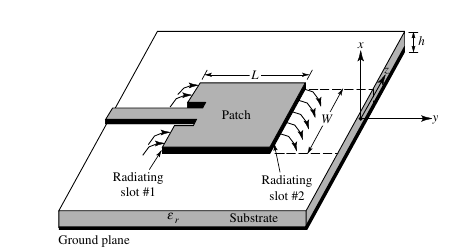
\includegraphics[scale=0.6]{micro.png}
	\caption{Antena Microcinta (Tomado de \cite{balanice}, pág. $812$).}
	\label{fig1}
\end{figure}
\noindent
El parche radiante puede ser cuadrado, rectangular, tira fina (dipolo), circular, elíptica, triangular, o puede ser cualquier otra configuración.\\
Existen muchas configuraciones que pueden ser utilizadas para alimentar antenas de Microcintas. Las cuatro más conocidas son: la línea Microcinta, la sonda coaxial, el acoplamiento de apertura y el acoplamiento de proximidad.

\subsection{Modelo de Línea de Transmisión}
\noindent
\textit{``Una antena microcinta rectangular se puede representar como un arreglo de dos aperturas radiantes estrechas (ranuras), cada una de anchura $W$ y altura $h$, separados por una distancia $L$. Básicamente el modelo de línea de transmisión representa la antena Microcinta por dos ranuras, separadas por una baja impedancia $Z_c$ y una línea de transmisión de longitud $L$''}\footnote{Balanice, Constantine A. 2005, ``Antenna theory analysis and desing'', \textit{John Wiley \& Sons, Inc.}, Third Edition, pág. $816$.}.\\
Este método utiliza las siguientes ecuaciones para determinar los parámetros físicos del arreglo:\\
Ecuación para determinar el ancho del parche:
\begin{equation}
  W_{opt}  = \frac{1}{2}\frac{{\lambda _0 }}{{\sqrt {\varepsilon _{average} } }}
\label{ecu1}
\end{equation}
\noindent
donde
\begin{equation*}
 \varepsilon _{average}  = \frac{1}{{\varepsilon _r  + 1}}
\end{equation*}
\noindent
Ecuación para determinar el valor de $\varepsilon _r$:
\begin{equation}
 \varepsilon _{erf}  = \frac{{\varepsilon _r  + 1}}{2} + \frac{{\varepsilon _r  - 1}}{{2\sqrt {1 + 12\frac{h}{W}} }}
\label{ecu2}
\end{equation}
\noindent
Ecuación para determinar la variación de la longitud:
\begin{equation}
 \Delta L = 0.412\frac{{\varepsilon _{erf}  + 0.3}}{{\varepsilon _{erf}  - 0.258}}\frac{{\frac{W}{h} + 0.264}}{{\frac{W}{h} + 0.8}}h
\label{ecu3}
\end{equation}
\noindent
Determinación de la longitud del parche:
\begin{equation}
 L_{patch} = \frac{{\lambda _g }}{2} - 2\Delta L = \frac{c}{{2\sqrt {\varepsilon _{erf} } }} - 2\Delta L
\label{ecu4}
\end{equation}
Ecuación para determinar la resistencia de entrada $R_{in}$:
\begin{equation}
 R_{in}  = \frac{1}{{2\left( {G_e  + G_{12} } \right)}}
\label{ecu7}
\end{equation}
\noindent
Donde:
\begin{equation}
 G_e  = \frac{{2{\mathop{\rm P}\nolimits} _{rad} }}{{\left| {V_0 } \right|^2 }} = \frac{{ - 2 + \cos \left( X \right) + XS_i \left( X \right) + \frac{{\sin \left( X \right)}}{X}}}{{120\pi ^2 }}
\label{ecu5}
\end{equation}
\noindent
donde:
$$X = k_0 W$$
$${S_i \left( X \right)} = \int\limits_0^X {\frac{{\sin u}}{u}du}$$

\begin{equation}
 G_{12}  = \frac{1}{{120\pi ^2 }}\int\limits_0^X {\left[ {\sin \frac{{k_0 W}}{2}\cos \theta } \right]} ^2 J_0 \left( {k_0 L\sin \theta } \right)\sin ^3 \theta d\theta
\label{ecu6}
\end{equation}

\subsection{Híbrido a $90°$}
\noindent
El híbrido en cuadratura o también llamado híbrido de $3\ dB$, es el tipo de híbrido fabricado en microcinta el cual utiliza una técnica de descomposición en modo par-impar similar a la utilizada en el divisor de potencia Wilkinson. La matriz de parámetros $[S]$ que caracteriza el comportamiento de este tipo de híbrido es de la siguiente forma:
$$
\left[ S \right] = \frac{{ - 1}}{{\sqrt 2 }}\left[ {\begin{array}{*{20}c}
   0 & j & 1 & 0  \\
   j & 0 & 0 & 1  \\
   1 & 0 & 0 & j  \\
   0 & 1 & j & 0  \\
\end{array}} \right]
$$
\noindent
Su funcionamiento radica en la gran simetría que presenta el dispositivo con lo que se pueden intercambiar sin problemas las entradas entradas y salidas, la potencia que ingresa por el puerto $1$ se divide por igual entre los puertos $2$ y $3$, con un desplazamiento de fase de $90°$ entre sus salidas y la alimentación no se encuentra acoplada al puerto $4$ que representa un puerto aislado.\\
El diseño de este tipo de híbridos en Microcinta es trivial, dado que sólo se debe fijar el valor de la impedancia de referencia y posterior a esto se calculan  el ancho de las pistas para las impedancias requeridas. Con ayuda de un programa de simulación como Qucs, se podrá calcular las dimensiones del híbrido a $90°$.En la Fig. \ref{fig100} se presenta la geometría para la construcción del  híbrido.
\begin{figure}[H]
	\centering
		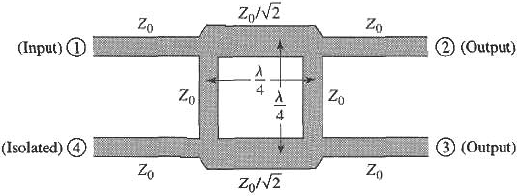
\includegraphics[scale=0.6]{hibrido.png}
	\caption{Geometría de un acoplador de Cuadratura (Híbrido de $90°$).}
	\label{fig100}
\end{figure}

\section{Descripción del Método}
\noindent
Dado que la antena debe funcionar a $f=5.8 \pm 1\%\ GHz$, el arreglo de antenas  rectangulares tipo parche debe tener una polarización ortogonal al eje del arreglo, además el arreglo debe tener dos puertos de entrada, uno para el patrón Suma y el otro para el patrón Diferencia.

\subsection{Diseño de las antenas tipo parche}
\noindent
Dadas la ecuación (\ref{ecu1}), se determino el ancho de la antena $W=15.8163\ mm$.\\
Para determinar la longitud de la antena, es necesario calcular la variación de la longitud descrita por la ecuación (\ref{ecu3}), para determinar la longitud de la antena se hace uso de la ecuación (\ref{ecu4}) dando como resultado $L=12.2391\ mm$.\\
Al obtener los valores $W$ y $L$, se calculo la impedancia de entrada del parche por medio de las ecuaciones (\ref{ecu5}), (\ref{ecu6}) y (\ref{ecu7}), dando como resultado $R_{in}=318.8869\ \Omega$.\\
Como ya se determino la impedancia de entrada del parche, es necesario hacer una acople a $50\ \Omega$, para ello se utilizo un acoplador a $\lambda/4$, para este caso se usaron dos acoples diferentes. El primer acople tiene una línea de transmisión con $Z_c=56.4700\ \Omega$, para lograr una acople a $100\ \Omega$ se adiciono una segunda línea de transmisión a $Z_c=31.6227$, esto se utilizo para cada parche con el fin de lograr una impedancia de $50\ \Omega$ al hacer el paralelo entre las líneas que alimentan las parejas de parches y así acoplarlas a la impedancia característica del híbrido.

\subsection{Diseño del Híbrido a $90°$}
\noindent
Como una de las especificaciones del proyecto es alimentar por medio de dos puertos, se utilizo un Híbrido a $90°$, como este solo genera un desface de $90°$ entre sus salidas, se adicionaron líneas para lograr el patrón Suma (La señal entra a todos los parches con la misma fase) y el patrón Diferencia (La señal de entrada llega con $180°$ de desface a 2 parches).\\
Los resultados del híbrido fueron los siguientes:
\begin{table}[H]
	\centering
\begin{tabular}{|c|c|c|}\hline
\textbf{Linea} & \textbf{$W$} & \textbf{$L$} \\ \hline
\textbf{Superior e Inferior} & $2.3169\ mm$ & $6.9355\ mm$ \\ \hline
\textbf{Laterales} & $1.346\ mm$ & $7.1433\ mm$ \\ \hline
    \end{tabular}
	\caption{Parámetros determinados por Qucs.}
	\label{tab1}
\end{table}
\noindent
Para poder cumplir el requerimiento de la alimentación por dos puertos y lograr los dos patrones, se adicionaron al final del híbrido (puertos $2$ y $3$) dos líneas de transmisión cuyas longitudes permitieran lograr los desfaces necesarios, uno de ellos es una línea a $180°$ y la otra a $90°$. Por medio de este sistema todo los componentes quedaron acoplados a $50\ \Omega$. Se decidió alimentar el híbrido en los puertos 1 y 4 con lineas de transmisión de $360°$ para cada puerto, con el fin de tener simetría en las entradas y una longitud practica para el proceso de implementación, ya que se busca comodidad para el acople de los conectores \textit{SMA} con el sistema.

\subsection{Diseño final del sistema Microcinta}
\noindent
Al tener todos los parámetros físicos del arreglo y del híbrido calculados, se realizó el diseño de toda la red de Microcinta en Autocad, con el fin de llevarlo a escala real ($1:1$) Fig \ref{fig5}.
\begin{figure}[H]
	\centering
		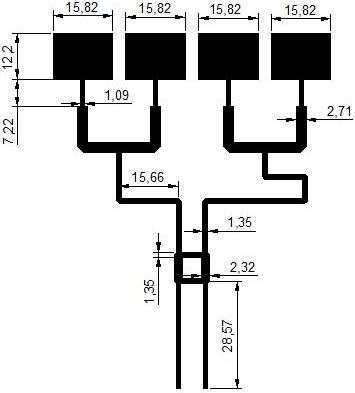
\includegraphics[scale=0.5]{esquema.jpg}
	\caption{Esquema diseñado en AutoCad a escala $1:2$ en $mm$.}
	\label{fig5}
\end{figure}

\section{Resultados de la Simulación}
\begin{figure}[H]
	\centering
		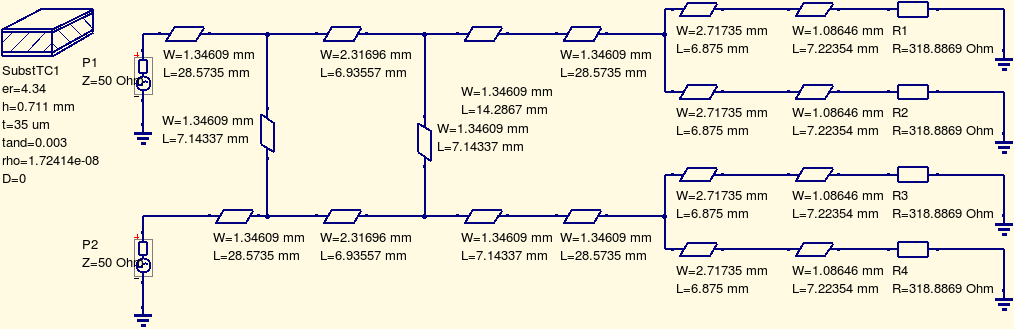
\includegraphics[scale=0.34]{qucs.png}
	\caption{Circuito Simulado en Qucs.}
	\label{fig6}
\end{figure}
\noindent
De acuerdo a los resultados obtenidos anteriormente se $\ $construyó el circuito de la Fig. \ref{fig6}, se obtuvieron los siguientes resultados:
\begin{figure}[H]
	\centering
		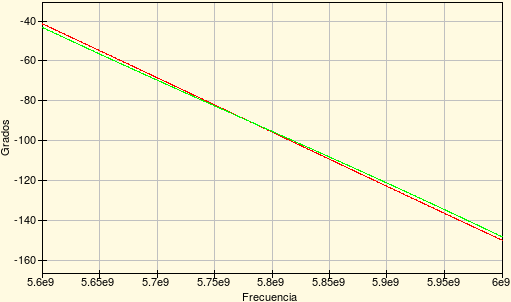
\includegraphics[scale=0.6]{suma.png}
	\caption{Ángulos de llegada a los parches para el patrón Suma simulado en Qucs.}
	\label{fig7}
\end{figure}

\begin{figure}[]
	\centering
		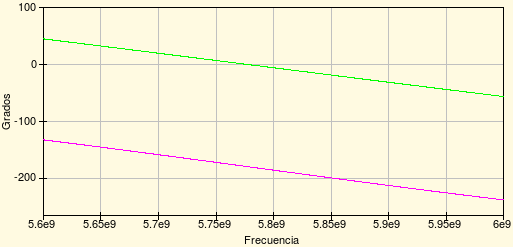
\includegraphics[scale=0.6]{resta.png}
	\caption{Ángulos de llegada a los parches para el patrón Diferencia simulado en Qucs.}
	\label{fig8}
\end{figure}
\noindent
Como se observa en la Fig. \ref{fig7} el ángulo con que llega la señal de entrada tiene un desface de $0°$ en casi todas las frecuencias de muestreo.\\ De la Fig. \ref{fig8} se observa que el ángulo de la señal de entrada a los parches es de $180°$ en todas las frecuencias de muestreo.
\begin{figure}[H]
	\centering
		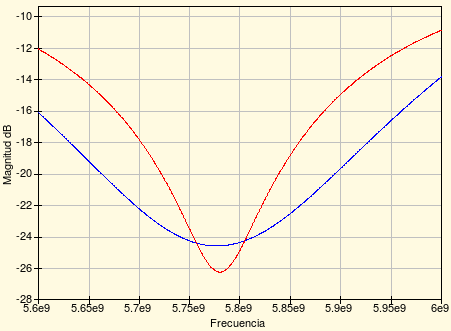
\includegraphics[scale=0.6]{paras.png}
	\caption{Ganancia del coeficiente de reflexión para el puerto Suma (Azul) y Diferencia (Rojo) simulado en Qucs.}
	\label{fig9}
\end{figure}
\noindent
En la Fig. \ref{fig9} se obtuvo la ganancia de los parámetros $S[1,1]$ y $S[4,4]$ del sistema para poder determinar que tanta eficiencia tiene el arreglo del híbrido a $90°$ para la distribución de potencia en el arreglo.\\
A partir a las simulaciones desarrolladas en Qucs se observa que la red diseñada cumple con las especificaciones requeridas de este proyecto, por ende se procedió al proceso de implementación; para la muestra de los lóbulos de los diferentes patrones de Suma/Diferencia, se procedió a realizar las simulaciones en Feko.

\subsection{Simulaciones en FEKO}
\noindent
Los resultados que se obtuvieron con el análisis anterior, se simularon en Feko para así visualizar todos los lóbulos característicos de cada patrón y por medio de estos identificar la ganancia máxima para el caso del patrón Suma, y en el caso del patrón Diferencia observar el nulo entre los dos lóbulos resultantes.\\
Las Figuras \ref{fig10} y \ref{fig11} muestran la radiación de los lóbulos de los patrones requeridos, con sus respectivas ganancias. Para este caso en particular el patrón Suma tiene una ganancia mayor que el patrón Diferencia, dado que tiene una mayor directividad.
\begin{figure}[H]
	\centering
		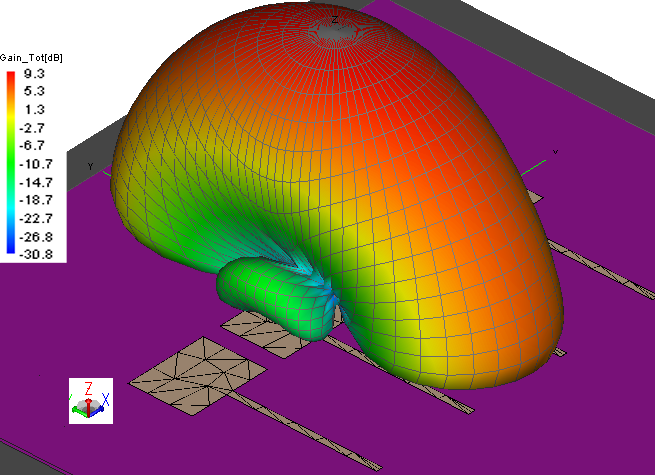
\includegraphics[scale=0.5]{sumafeko.png}
	\caption{Ganancia de la antena para el patrón Suma simulado en Feko.}
	\label{fig10}
\end{figure}
\begin{figure}[H]
	\centering
		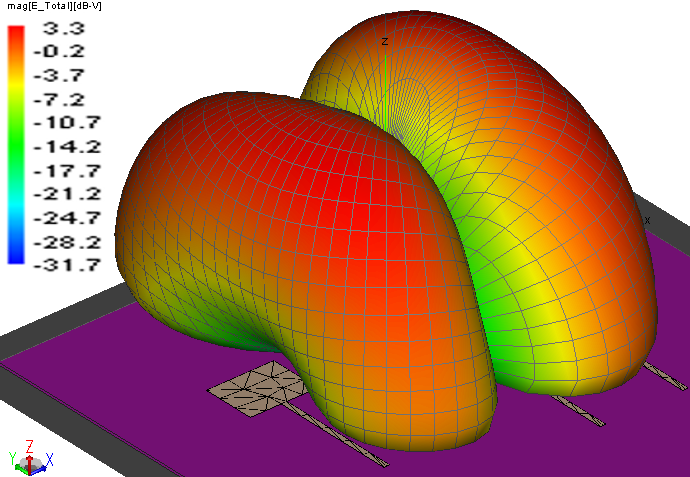
\includegraphics[scale=0.5]{restafeko.png}
	\caption{Ganancia de la antena para el patrón Diferencia simulado en Feko.}
	\label{fig11}
\end{figure}
\noindent
A continuación se muestra la curva de la ganancia en función de la frecuencia para el caso del patrón Suma.
\begin{figure}[H]
	\centering
		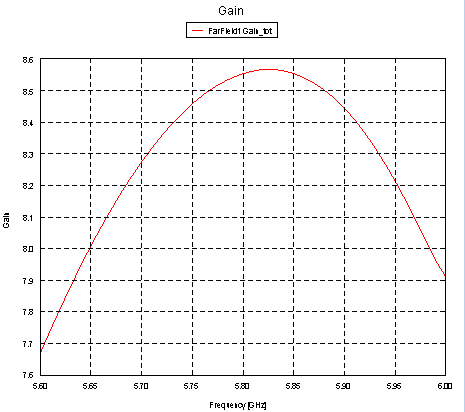
\includegraphics[scale=0.62]{gan_suma.png}
	\caption{Ganancia de la antena del patrón Suma en dB simulado en Feko.}
	\label{fig12}
\end{figure}
\noindent
La ganancia es máxima aproximadamente en $5.82\ GHz$ obteniendo un valor máximo de $8.575\ dB$. Una de las especificaciones del proyecto era obtener una ganancia superior a $10\ dB$, se considero que aunque el resultado por simulación no supero este valor (ver Fig. \ref{fig11}) es importante mencionar que para el arreglo de antenas en patrón Suma se tiene un arreglo Broad-Side para el cual, debido a la influencia del plano de tierra el promedio del patrón de ganancia ya no estará ubicado en el origen si no que se vera incrementado en $3\ dB$ de ganancia, por este motivo se considera que la ganancia final sera de un valor aproximado de $11\ dB$.
\begin{figure}[H]
	\centering
		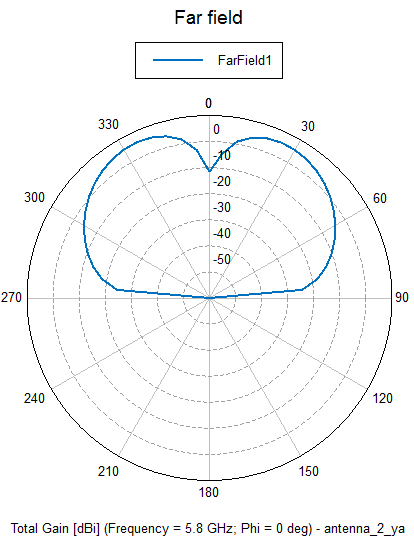
\includegraphics[scale=0.62]{ganancia.png}
	\caption{Ganancia de patrón Diferencia simulado en Feko.}
	\label{fig13}
\end{figure}
\noindent
La ganancia del patrón diferencia observada en la Fig. \ref{fig13} muestra que el ancho máximo del nulo es inferior a $15°$ cuando se evalúa $-6\ dB$ por debajo  del punto máximo de los lóbulos laterales.

\section{Conclusiones}
\begin{itemize}
 \item Como se observo en las simulaciones el patrón Suma tiene una mayor directividad con respecto al patrón Diferencia, en el caso de la Suma se comporta como un arreglo en Broad-Side con unos lóbulos laterales muy pequeños inferiores a $-13\ dB$. Por otro lado en el caso del patrón Diferencia tanto la directividad como la ganancia son menores y la separación de los lóbulos laterales en el punto de $-6\ dB$ es inferior a $15°$ lo que es útil para aplicaciones que requieran recepción.
\end{itemize}

\bibliographystyle{ieeetran}
\begin{thebibliography}{99}

\bibitem{balanice} Balanice, Constantine A. 2005
{\em ``Antenna theory analysis and desing''}, \textit{John Wiley \& Sons, Inc.}, Third Edition.

\bibitem{page1} Feko ``Feko User's Manual'', en línea, 21 Npviembre de 2010, Disponible en \url{http://people.ee.ethz.ch/~fieldcom/pps-antenna/doc/UserManual.pdf}.

\end{thebibliography}
\end{document}